\chapter{Metodología y Desarrollo del Sistema}

\section{Proceso de desarrollo}

El desarrollo se organizó alrededor de las funciones del sistema: catálogo, autenticación, inventario, compras, ventas y seguimiento de pedidos. El repositorio incluye migraciones para el esquema de datos, controladores y vistas por módulo, seeders para poblar los usuarios y el catálogo, y pruebas automatizadas de diferentes flujos. Git permite versionar el código y coordinar cambios entre integrantes del equipo \cite{git_scm}.

La preparación del esquema se realiza con migraciones de Laravel. Los seeders del proyecto cargan usuarios y datos de catálogo; el seeder curado permite restaurar productos e imágenes. El comando \texttt{catalogo:exportar-seeder} exporta datos e imágenes al formato versionado por el proyecto. El proceso de sincronización está cubierto por pruebas de integración.

\section{Arquitectura de la infraestructura multi-contenedor}

El archivo \texttt{docker-compose.yaml} declara tres servicios con nombres de contenedor explícitos, conectados a la red privada \texttt{archivum-net}. La configuración usa volúmenes para persistir la base de datos y compartir las dependencias y los recursos frontend compilados.

\begin{table}[htbp]
\centering
\caption{Servicios declarados en la configuración Docker Compose de Archivum.}
\label{tab:infraestructura_docker}
\begin{tabularx}{\textwidth}{|l|l|l|X|}
\hline
\textbf{Contenedor} & \textbf{Imagen/base} & \textbf{Puerto} & \textbf{Función configurada} \\ \hline
\texttt{archivum\_app} & \texttt{php:8.4-fpm} & 9000 interno & Ejecuta Laravel con PHP-FPM y se conecta a MariaDB por la red de Compose. \\ \hline
\texttt{archivum\_db} & \texttt{mariadb:11.2} & 3306 interno & Almacena la base de datos; usa el volumen \texttt{db\_data} y una comprobación de salud. \\ \hline
\texttt{archivum\_nginx} & \texttt{nginx:alpine} & 8000:80 & Recibe las solicitudes HTTP y reenvía las solicitudes PHP a \texttt{app:9000}. \\ \hline
\end{tabularx}
\end{table}

El Dockerfile instala las extensiones PHP requeridas por el proyecto y crea el usuario \texttt{archivum} con UID y GID 1000. El servicio de base de datos declara el usuario numérico 999:999. Al iniciar, el comando de aplicación prepara el archivo de entorno si falta, genera la clave, ejecuta las migraciones y arranca PHP-FPM. La instrucción reproducible de arranque declarada es:

\begin{verbatim}
docker compose up -d --build
\end{verbatim}

\section{Modelo de datos y relaciones}

El esquema está definido en las migraciones de \texttt{database/migrations/}. La organización siguiente agrupa las tablas por responsabilidad y resume las relaciones principales.

\subsection{Usuarios, roles y auditoría}

\begin{itemize}
    \item \texttt{usuarios}: cuentas, correo, contraseña, estado activo y eliminación lógica.
    \item \texttt{roles} y \texttt{usuario\_rol}: catálogo y relación muchos a muchos de roles y usuarios.
    \item \texttt{recuperacion\_contrasenas}: token con hash, vencimiento y fecha de uso.
    \item \texttt{clientes}, \texttt{direcciones} y \texttt{clientes\_frecuentes}: perfil comercial, direcciones y datos de fidelización.
    \item \texttt{bitacoras}: actor, acción, tabla afectada, registro, detalle e IP.
\end{itemize}

\subsection{Catálogo y especializaciones}

\begin{itemize}
    \item \texttt{catalogos} clasifica los productos; \texttt{productos} almacena nombre, descripción, precio y estado.
    \item \texttt{libros} añade ISBN, autor, editorial, año de publicación y páginas.
    \item \texttt{discos} añade artista, sello, género, formato, año de lanzamiento e imagen.
    \item \texttt{coleccionables} añade marca, serie, material, indicador de edición limitada e imagen.
    \item \texttt{variantes\_sku} define la clave SKU única y su descripción y precio opcional.
    \item \texttt{promociones} y \texttt{cliente\_promocion} almacenan promociones y su relación con clientes.
\end{itemize}

Cada tabla de especialización se vincula mediante \texttt{producto\_id}; las existencias y variantes se mantienen en entidades separadas. En las migraciones consultadas, los campos de condición detallada no aparecen en todas las categorías: la singularidad se registra mediante \texttt{piezas\_unicas}, con número de serie, certificado, notas y estado.

\subsection{Sucursales, existencias y movimientos}

\texttt{sucursales} representa las ubicaciones. \texttt{existencias} vincula una variante SKU con una sucursal y guarda cantidad y nivel mínimo; una restricción única impide duplicar esa pareja. \path{piezas_unicas} individualiza ejemplares asociados a una existencia. \path{movimientos_inventario} registra existencia, usuario, tipo, cantidad, motivo y referencia polimórfica. Los tipos definidos son entrada, salida, ajuste, traspaso y devolución.

\subsection{Carritos, reservas, pedidos y pagos}

\texttt{carritos} se relaciona con clientes y \texttt{carrito\_items} con variantes SKU. \texttt{reservas\_stock} se asocia a una existencia y puede vincularse con carrito o pedido; registra cantidad, vencimiento y estado. El código de checkout define una duración de cinco minutos para las reservas temporales.

\texttt{pedidos} almacena folio, cliente, dirección de envío, estado y montos. \texttt{detalle\_pedidos} relaciona pedido y variante, y conserva el precio unitario aplicado. \texttt{pagos} y \texttt{detalle\_pagos} registran los datos de pago y sus detalles. \texttt{devoluciones} enlaza pedido, cliente y detalle para registrar la solicitud y su estado.

\subsection{Envíos, proveedores y contacto}

\texttt{envios}, \texttt{detalle\_envios} e \texttt{historial\_envios} modelan los datos del envío y su historial. \texttt{proveedores} almacena los datos de contacto y se relaciona con \texttt{movimientos\_inventario} mediante \texttt{proveedor\_id}. \texttt{mensajes\_contacto} almacena los mensajes recibidos desde el portal.

El módulo de compras presenta recepciones de mercancía a partir de movimientos de inventario de tipo entrada. En las migraciones no hay una tabla independiente de órdenes de compra; por tanto, el documento describe esa función como recepción de proveedor y no como ciclo persistente de órdenes con partidas.

\section{Implementación de módulos funcionales}

\subsection{Portal público, catálogo y búsqueda}

\texttt{CatalogoPublicoController} ofrece páginas para libros, discos, coleccionables y adquisiciones selectas. El catálogo permite buscar por texto y filtrar, según sección, por género de libro, formato de disco o categoría de coleccionable. La búsqueda considera campos generales, SKU y metadatos seleccionados como autor, ISBN, artista y sello. La consulta limita los resultados a productos activos y usa la sucursal pública resuelta por la aplicación.

\begin{figure}[htbp]
    \centering
    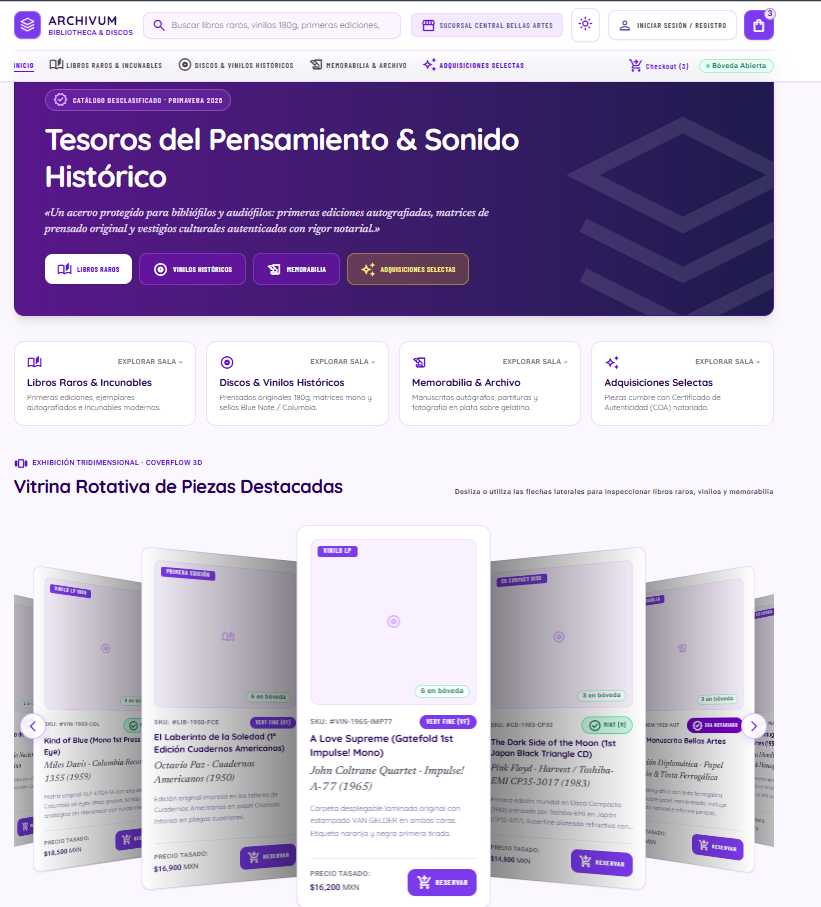
\includegraphics[width=0.88\textwidth,height=0.65\textheight,keepaspectratio]{imagenes/interfaz_publica.png}
    \caption{Catálogo público de Archivum.}
    \label{fig:interfaz_publica_archivum}
\end{figure}

\subsection{Autenticación, perfiles y roles}

Las rutas de invitado incluyen registro, inicio de sesión y solicitud de restablecimiento de contraseña; las rutas autenticadas permiten actualizar perfil y contraseña. El restablecimiento utiliza tokens con vencimiento. El middleware de autorización verifica los roles y existen controles adicionales de acceso por sucursal y de propiedad de pedidos o carritos.

\begin{figure}[htbp]
    \centering
    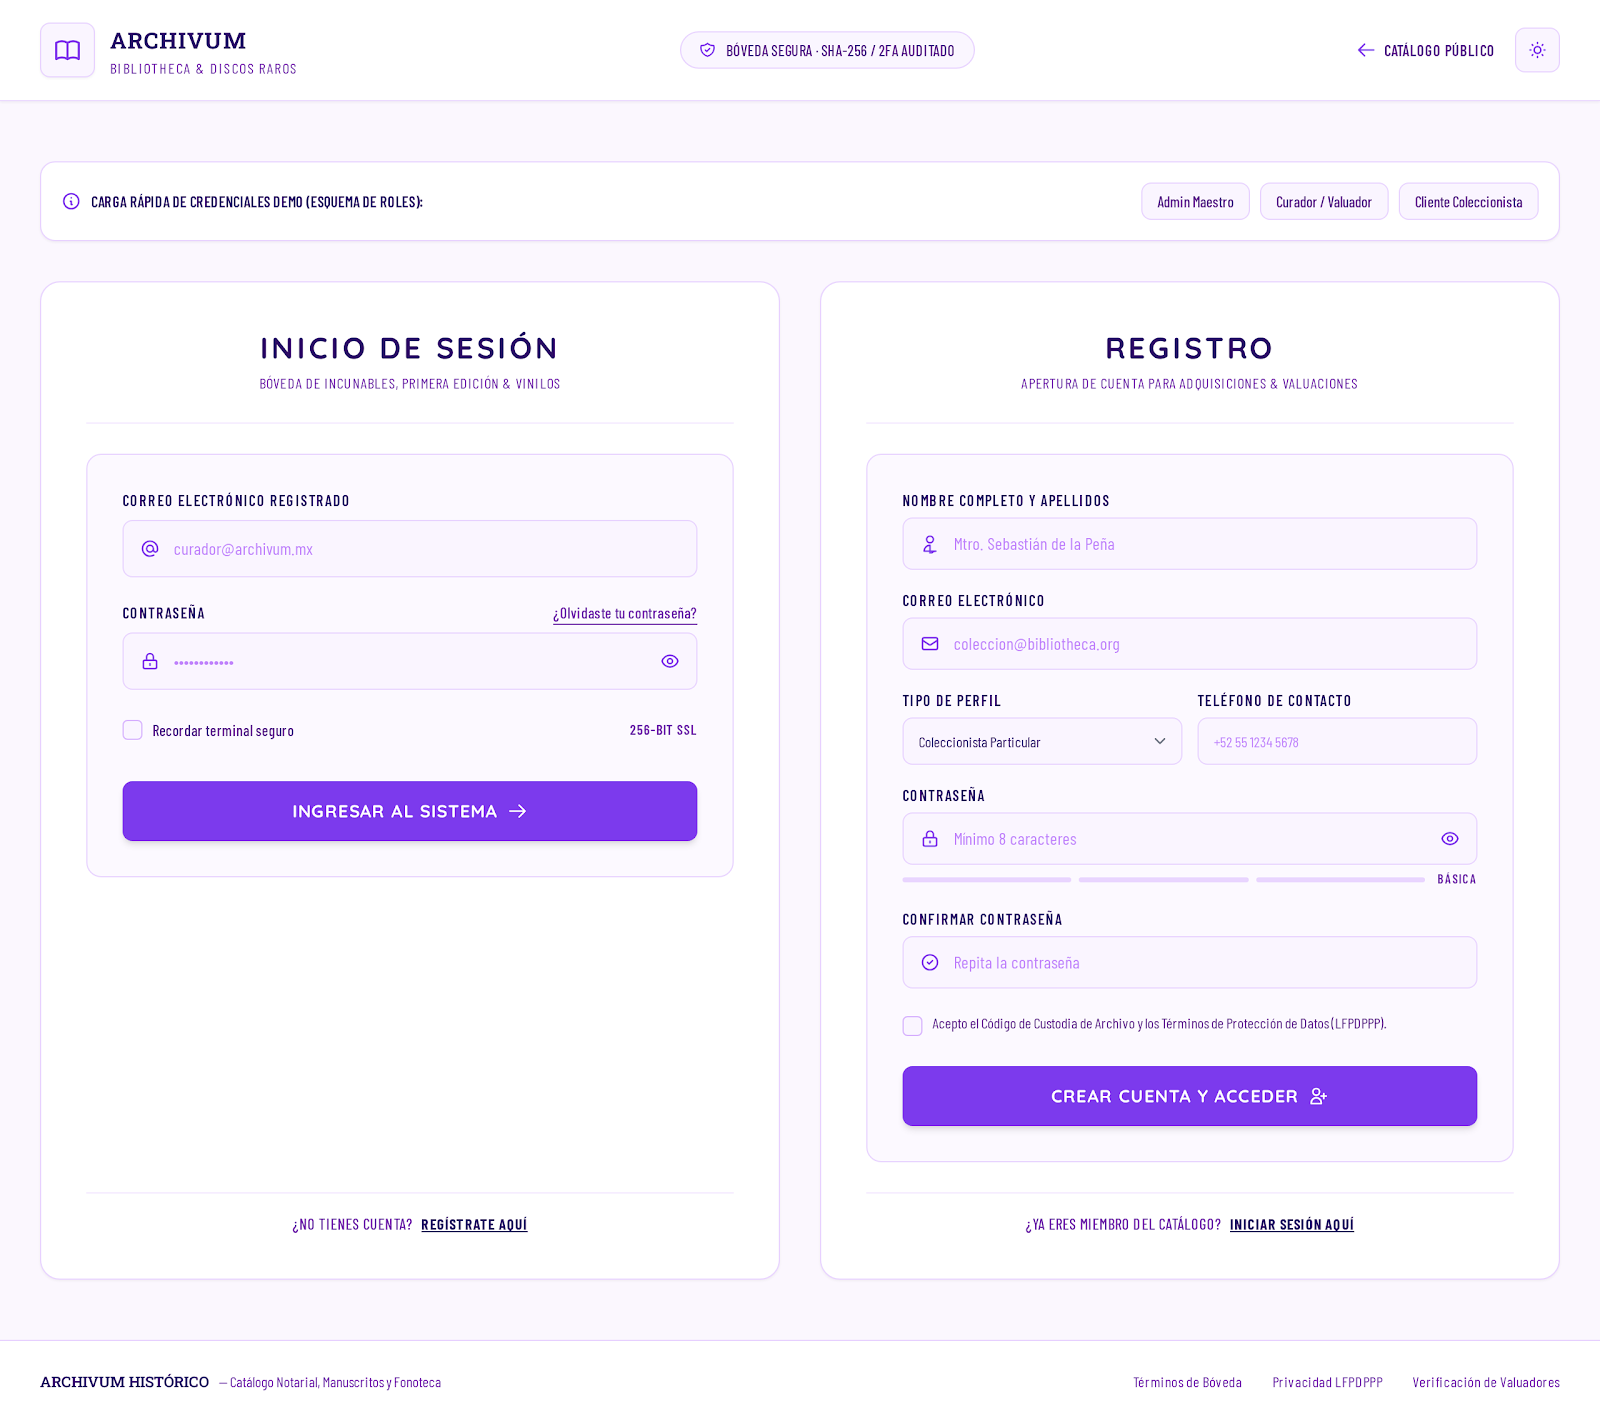
\includegraphics[width=0.82\textwidth,height=0.65\textheight,keepaspectratio]{imagenes/auth_registro.png}
    \caption{Interfaz de acceso y registro de clientes.}
    \label{fig:auth_registro}
\end{figure}

El seeder inicial crea los roles administrador, ventas, almacén, compras y cliente. Algunas rutas contemplan también \texttt{encargado}; como este perfil no se crea en el seeder inicial, se documenta como una opción reconocida por parte de la autorización, no como rol inicial poblado.

\subsection{Carrito, reservas y checkout simulado}

\texttt{CheckoutSimuladoController} gestiona la incorporación, actualización y eliminación de productos del carrito, la consulta del checkout, la confirmación del pedido y algunos estados de envío. La reserva temporal se implementa en el flujo de carrito y se libera cuando vence; el middleware \texttt{reservas.liberar} participa en su mantenimiento. La vigencia definida por el código es de cinco minutos. El pago es simulado y no acredita la conexión con una pasarela externa ni una garantía de serialización bajo carga concurrente.

\begin{figure}[htbp]
    \centering
    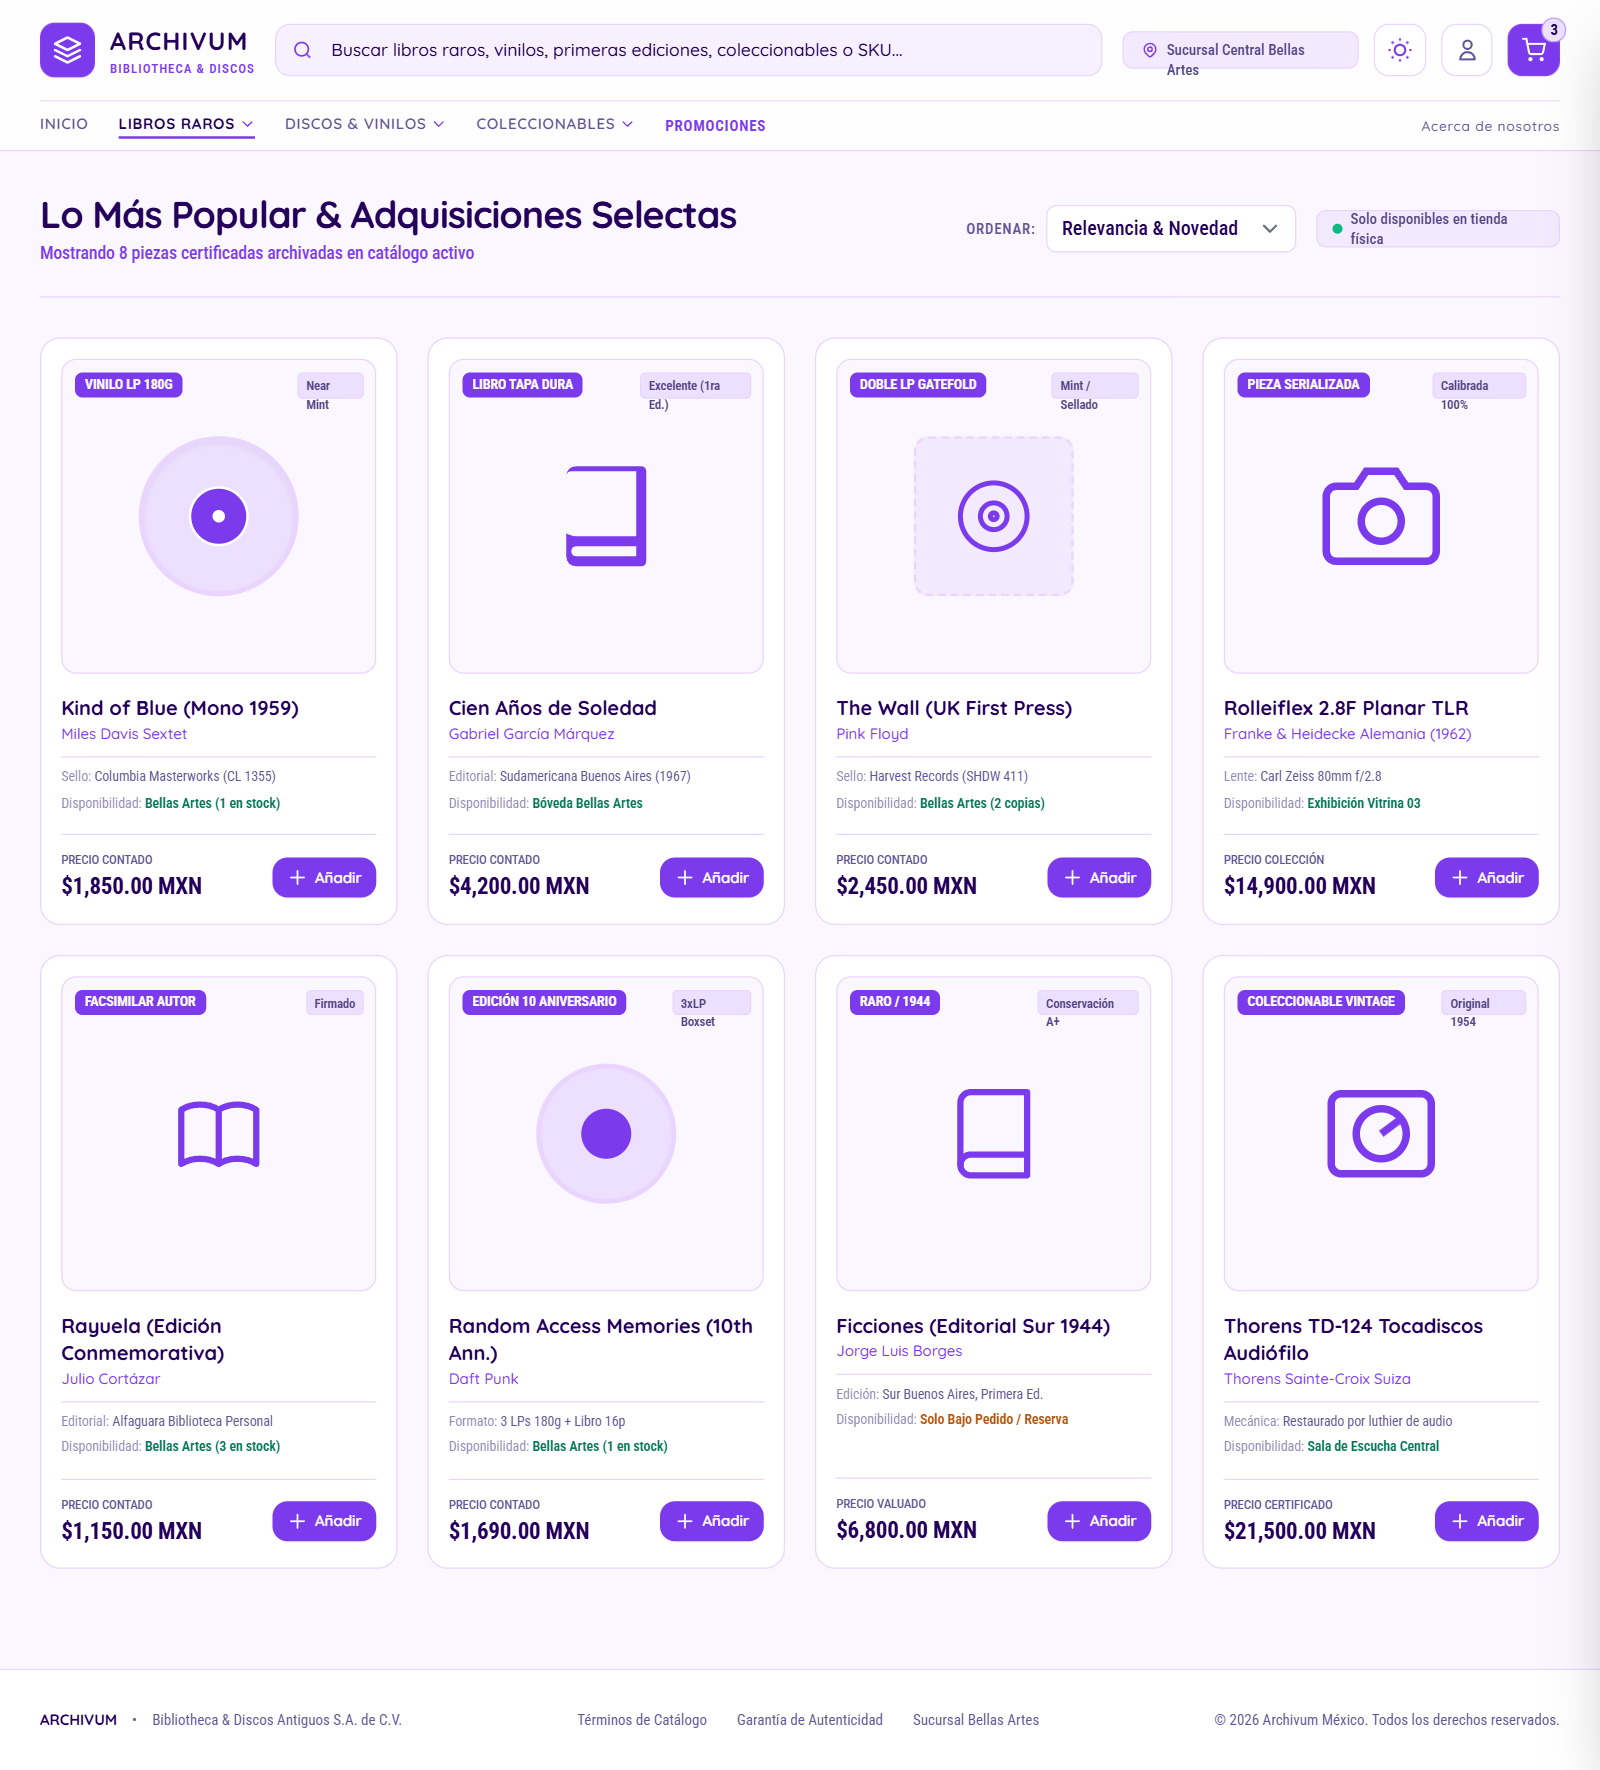
\includegraphics[width=0.88\textwidth,height=0.65\textheight,keepaspectratio]{imagenes/carrito_compras.png}
    \caption{Catálogo y carrito de compras.}
    \label{fig:carrito_archivum}
\end{figure}

\begin{figure}[htbp]
    \centering
    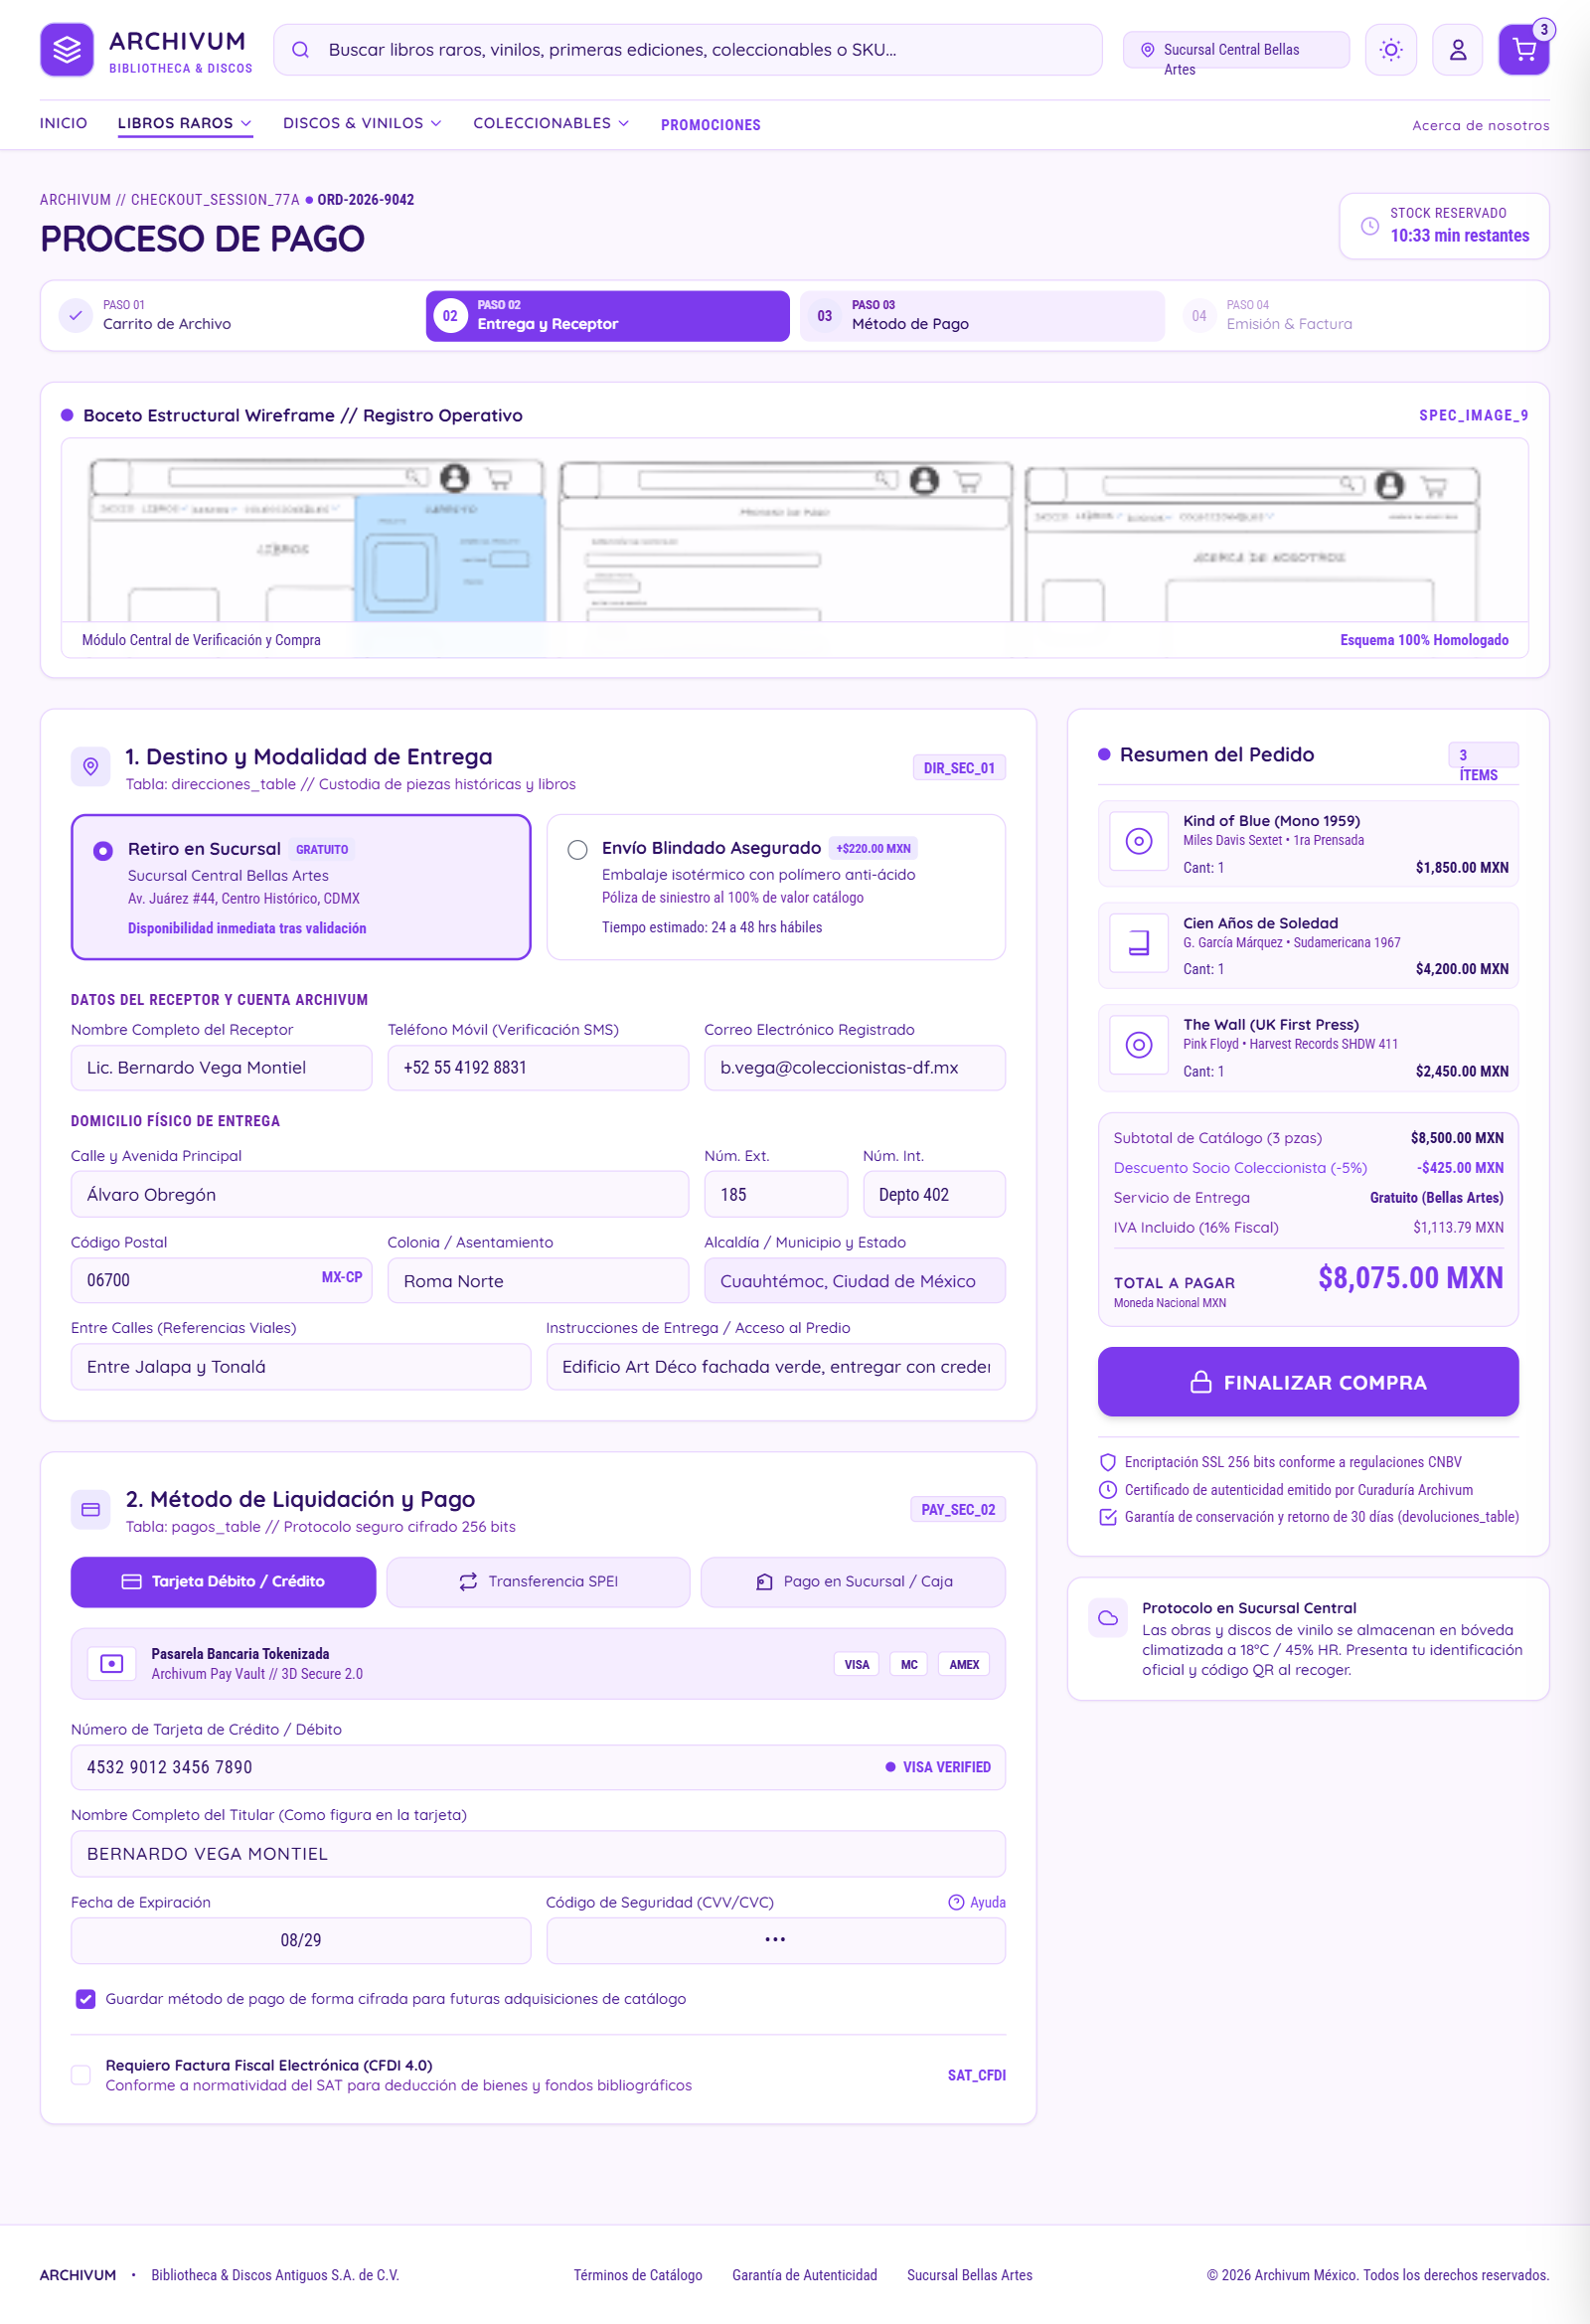
\includegraphics[width=0.88\textwidth,height=0.65\textheight,keepaspectratio]{imagenes/checkout_proceso.png}
    \caption{Flujo de checkout simulado.}
    \label{fig:checkout_archivum}
\end{figure}

\subsection{Panel administrativo, inventario y sucursales}

El área administrativa proporciona vistas para el tablero, empleados, roles, bitácora, reportes, mensajes, sucursales e inventario. El inventario se consulta por variante y sucursal, con filtros y alertas basadas en el stock mínimo. El personal puede registrar ajustes y movimientos de entrada o salida; las transferencias se registran como traspasos y el destino confirma su recepción. La aplicación ofrece también vistas para envíos y ventas.

\begin{figure}[htbp]
    \centering
    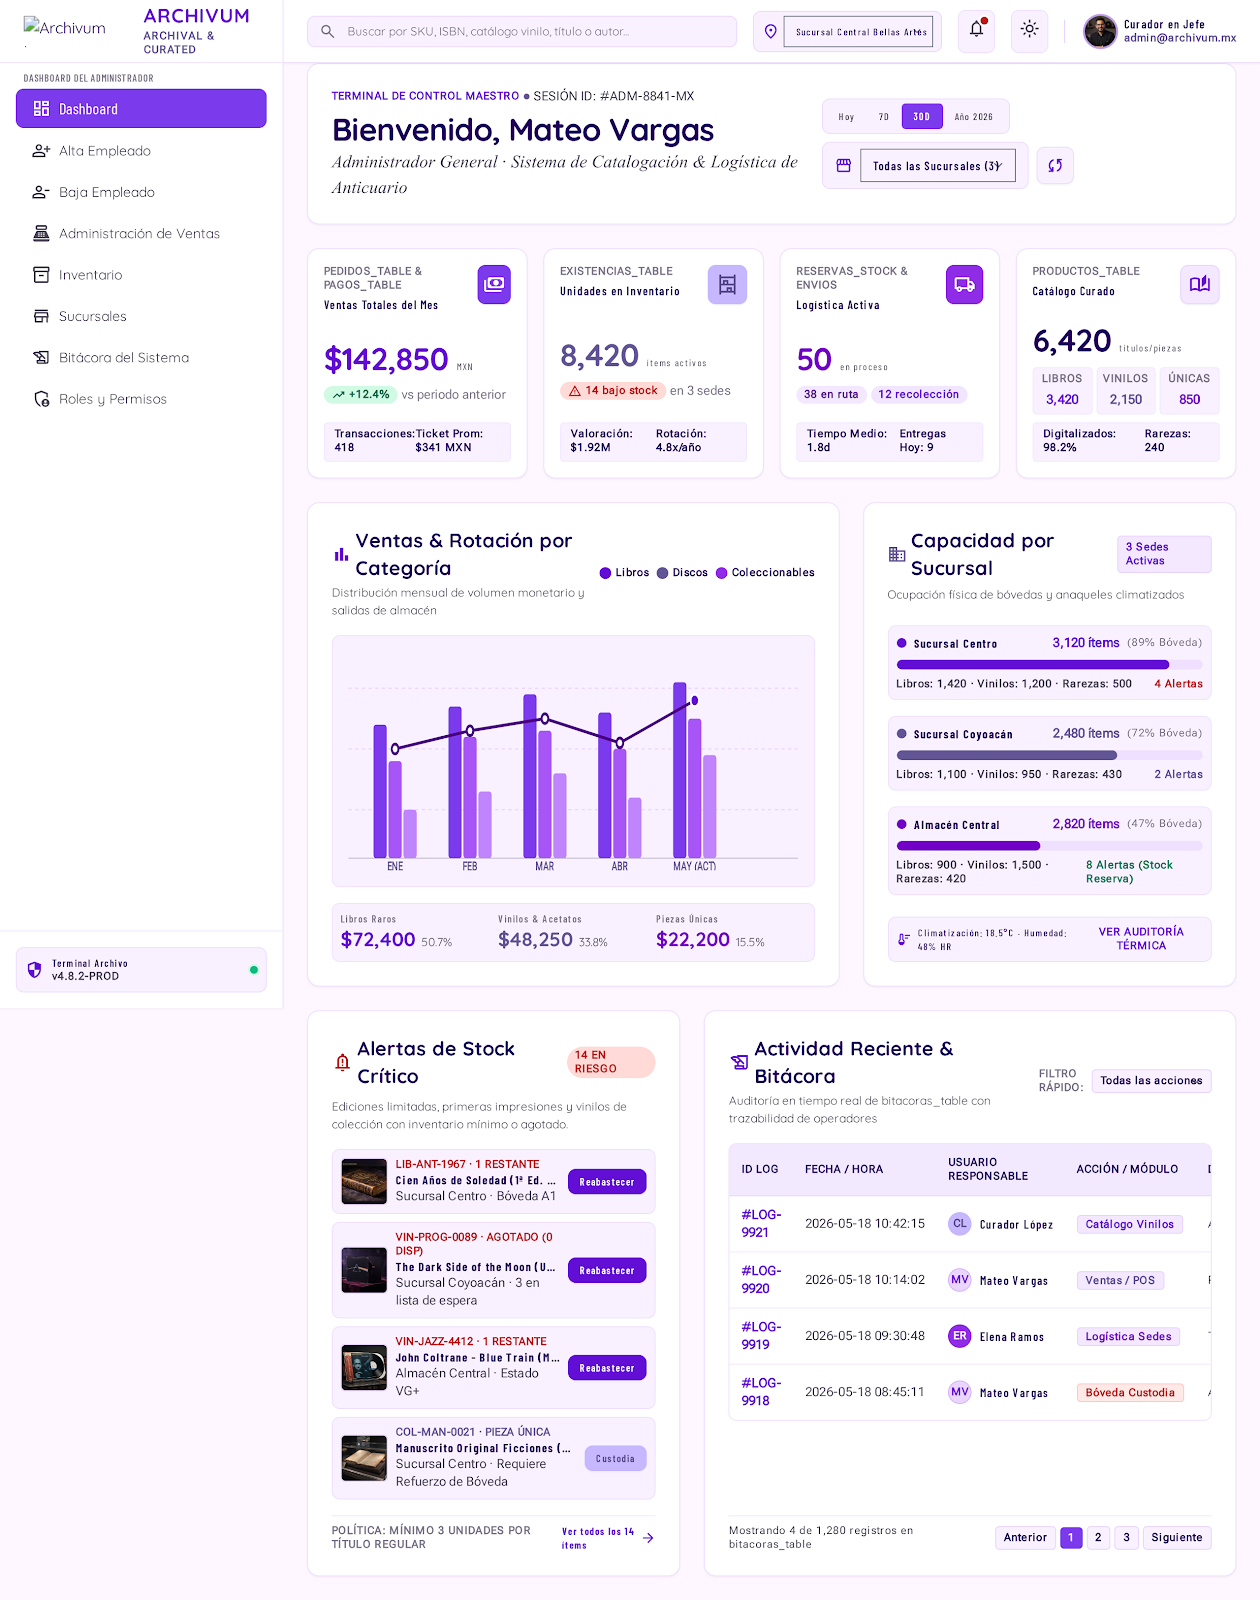
\includegraphics[width=0.88\textwidth,height=0.65\textheight,keepaspectratio]{imagenes/dashboard_admin.png}
    \caption{Panel administrativo de Archivum.}
    \label{fig:dashboard_archivum}
\end{figure}

\begin{figure}[htbp]
    \centering
    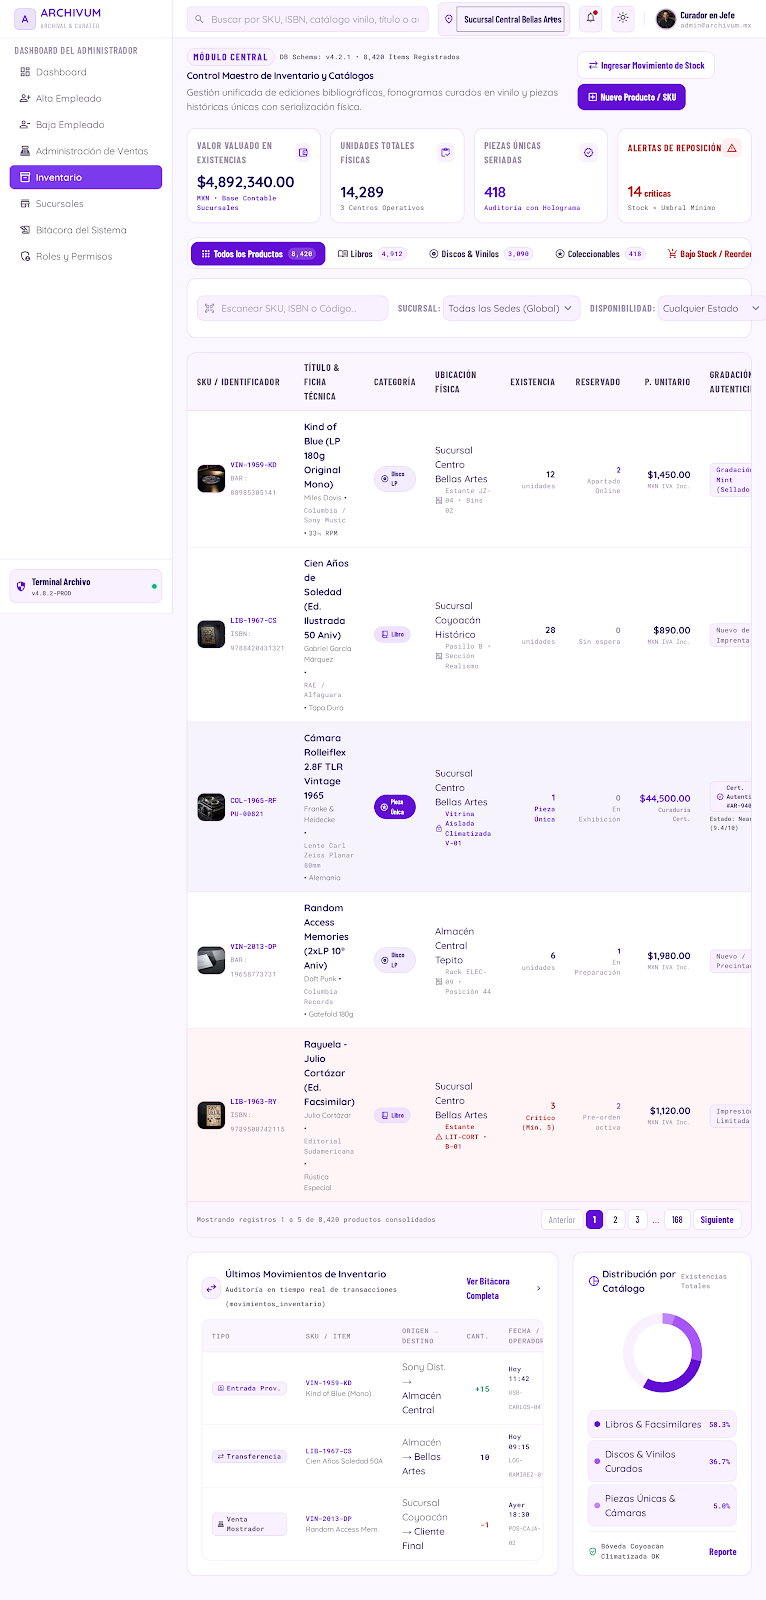
\includegraphics[width=0.88\textwidth,height=0.65\textheight,keepaspectratio]{imagenes/inventario_unificado.png}
    \caption{Consulta de inventario por sucursal.}
    \label{fig:inventario_archivum}
\end{figure}

\subsection{Proveedores, recepción, ventas y devoluciones}

El módulo de compras mantiene el directorio de proveedores, permite dar de alta productos y registrar recepciones que incrementan el inventario y generan movimientos. También incluye importación de productos por CSV. El área de ventas presenta pedidos, pagos, promociones y devoluciones; el personal autorizado puede cambiar estados y tramitar el dictamen y recepción de devoluciones. Los reportes administrativos se exportan en CSV y PDF.

\subsection{Sincronización del catálogo curado}

El comando \texttt{catalogo:exportar-seeder} exporta productos, variantes, existencias, metadatos e imágenes a los recursos versionados del seeder. \texttt{CatalogoCuradoSeeder} recrea los registros y sincroniza imágenes con los directorios utilizados por la aplicación. La prueba \texttt{SincronizacionCatalogoSeederTest} verifica exportación, restauración e idempotencia.

\subsection{Interfaz y experiencia de usuario}

Las vistas están implementadas con Blade y componentes compartidos para cabeceras, tarjetas, navegación y elementos de interfaz. Tailwind CSS aporta las clases de presentación y Vite compila los recursos frontend. Los layouts públicos y administrativos contemplan tema claro y oscuro, guardan la elección en el almacenamiento local del navegador y consultan la preferencia del sistema cuando no existe una preferencia guardada.
